% !TeX spellcheck = en_US
\addscenariosection{1}{Clash Scenario}{Dragon Valley}{\images/dragon.png}

\begin{multicols*}{2}

\textbf{Author:} LAAMAKALA

\textit{A valley of secrets long forgotten. Its heart belongs to the beasts of old, while its fringes lure the bold and the desperate. Fight for power, claim the land, or perish like those before you.}

\subsection*{\MakeUppercase{Scenario Length}}
This Scenario plays out over 13 Rounds.

\subsection*{\MakeUppercase{Player Setup}}
\textbf{Player Count:} 2 -- 4

\textbf{Starting Resources:} 14 \svg{gold}, 4 \svg{building_materials}, 1 \svg{valuables}

\textbf{Starting Income:} 10 \svg{gold}, 0 \svg{building_materials}, 0 \svg{valuables}

\textbf{Starting Units:}

\begin{itemize}
  \item A Pack of cheapest \bronze\ Units
  \item A Few chosen \bronze\ Units
\end{itemize}

\textbf{Town Buildings:}
\begin{itemize}
  \item \bronze\ Dwelling
  \item Each player may build the \svg{building_special_tent} building at a discount of 4 \svg{gold} and 2 \svg{building_materials}.
\end{itemize}

\textbf{Map Tile Pool:} Each player takes 3 Far (II–III) Map Tiles.

\subsection*{\MakeUppercase{Map Setup}}
Take the following Map Tiles ($P$ stands for the number of players) and arrange them as shown in the Scenario map layout:

\begin{itemize}
  \item P × Starting (I) Map Tile

  \item 2P × Near (IV–V) Map Tiles
  \item P × Center (VI–VII) Map Tile
  \item 1 × Center (VI–VII) Map Tile with a Dragon Utopia
\end{itemize}

\textbf{Additionally, for 4 players:}
\begin{itemize}
  \item 1 × Center (VI–VII) Map Tile with a Dragon Utopia
\end{itemize}

\subsection*{\MakeUppercase{Victory Conditions}}
The game ends at the end of the Round when any of the following conditions are met:

\begin{itemize}
 \item One player has defeated each other player's Main Heroes once. \textit{That player wins the game immediately.}
 \item One player has conquered both Dragon Utopias. \textit{That player wins the game immediately.}
 \item At the end of Round 13.
\end{itemize}

If no player achieves immediate victory, the player controlling a Dragon Utopia wins.
If different players control the two Utopias, they each draw Cards up to their Hand Limit and engage in a final Combat -- the winner is the victor.
If no one controls a Dragon Utopia, all players lose.
\subsection*{\MakeUppercase{Timed Events}}

\textbf{\nth{2} Round:}
\begin{itemize}
  \item Recruit one of your Units that has died for free.
\end{itemize}
\textbf{\nth{4} Round:}
\begin{itemize}
  \item Remove all Black Cubes from the Map.
\end{itemize}
\textbf{\nth{8} Round:}
\begin{itemize}
  \item Remove all Black Cubes from the Map.
\end{itemize}
\textbf{End of \nth{10} Round:}
\begin{itemize}
  \item The player(s) whose Main Hero has the least \svg{experience} roll(s) 2~\svg{resource}.
\end{itemize}

\subsection*{\MakeUppercase{Additional Rules}}
\begin{itemize}
  \item \textbf{Grail Token}: When a player gains or starts their turn with it, they gain +1 \svg{morale_positive} and Search (4) \svg{spellpower} or \svg{artifact}. Both Main and Secondary Heroes may pick up the Grail Token.
  \item Level VII Neutral Combats cannot be skipped.
  \item A defeated Main Hero may Empower one Defense Statistic Card from his M\&M Deck and gain +1 \svg{movement} for the next Round.
  \item After winning a Combat against another player's Main Hero, draw up to your Hand Limit and discard 1 Card.
  \item Level VII \textbf{Settlements/Random Town}: Increase all incomes by 1 space, Draw 2 Cards and gain +1 \svg{movement}.
  \item \textbf{Dragon Utopias} are guarded only by dragons.
  \item Upon flagging a \textbf{Dragon Utopia}, choose one option and then put a Black Cube:
  \begin{itemize}
    \item Gain 5 \svg{gold} and sacrifice any number of Units, then recruit one of the defeated dragons at a discount equal to the total recruitment cost of the sacrificed Units (to a minimum of 0).
    \item Gain 15 \svg{gold} and Search (3) \svg{spellpower} or \svg{artifact}.
  \end{itemize}
\end{itemize}

\begin{center}
  \vspace*{\fill}
  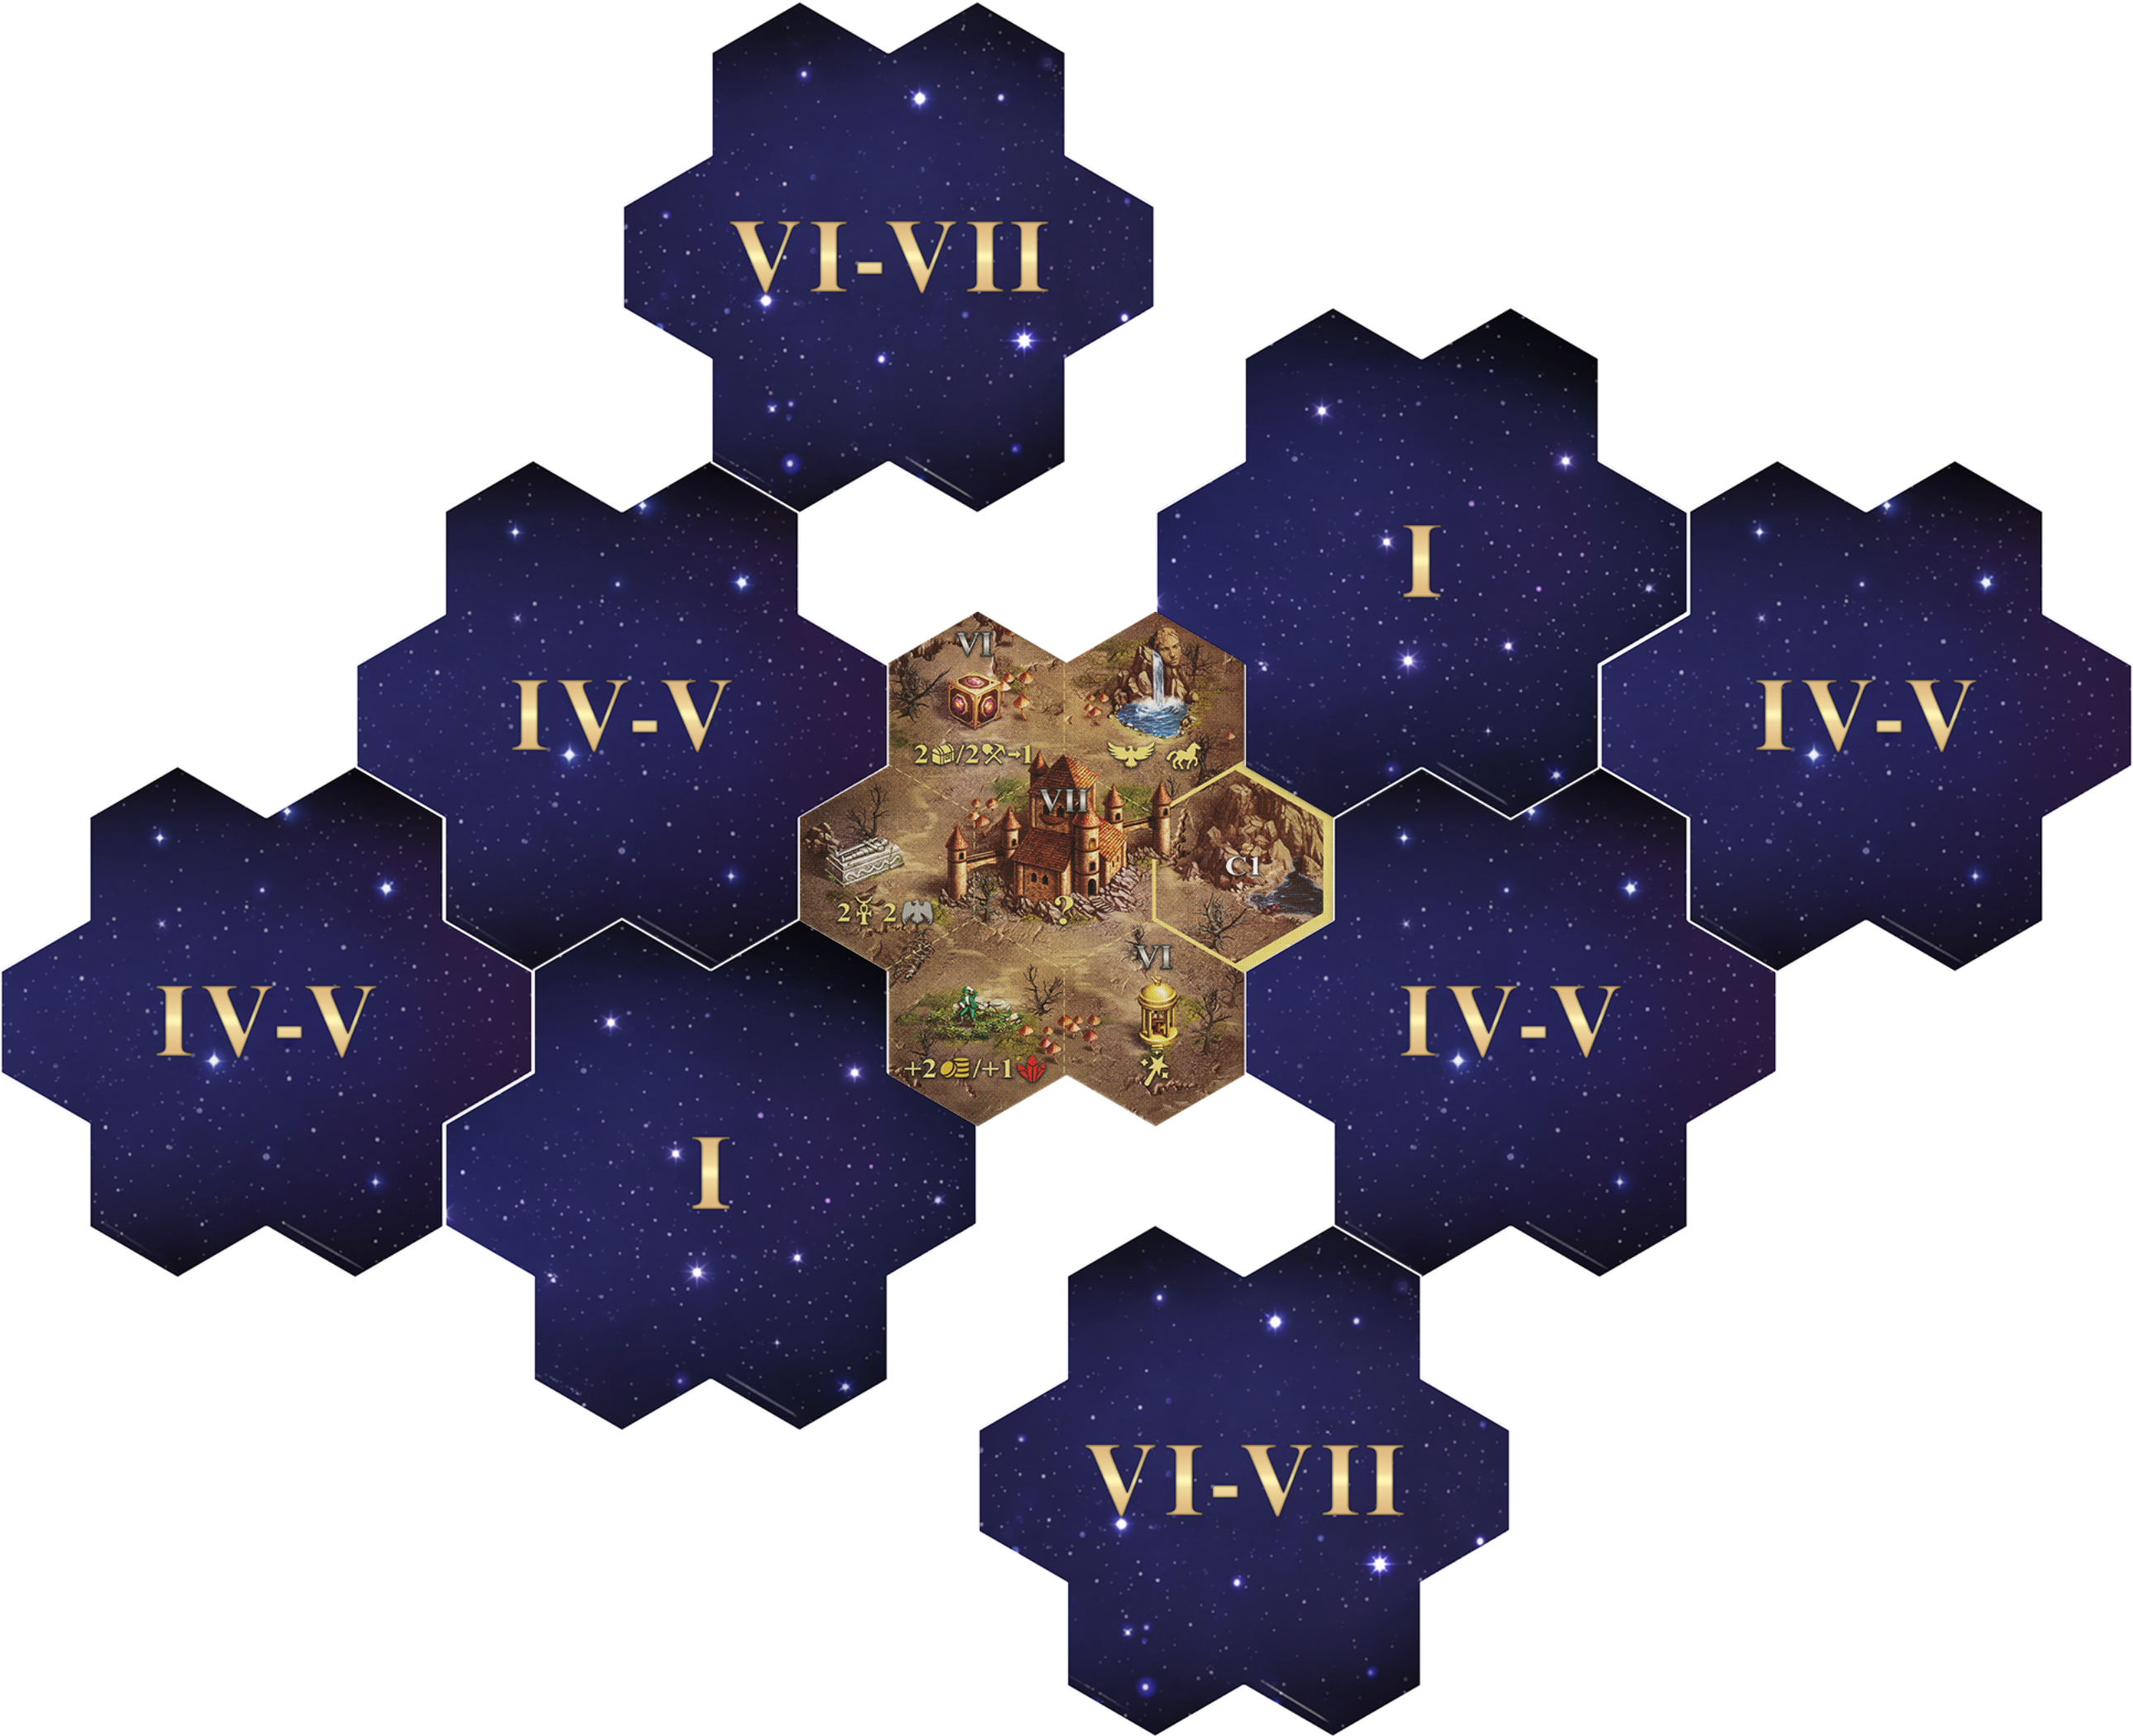
\includegraphics[width=0.8\linewidth]{\maps/dragon-valley-2p.png}
  \captionof{figure}{\textbf{2-PLAYER SCENARIO}}
\end{center}

\begin{itemize}
  \item When a \textbf{Secondary Hero} is recruited, you gain an additional Empowerment and one of each: Attack, Defense, and Power Statistic Cards, and a Magic Arrow. These may only be used by your Secondary Hero.
  \item When a Secondary Hero starts their turn on a I or II--III Map Tile, they gain +1~\svg{movement}.
\end{itemize}

\begin{center}
  \vspace*{\fill}
  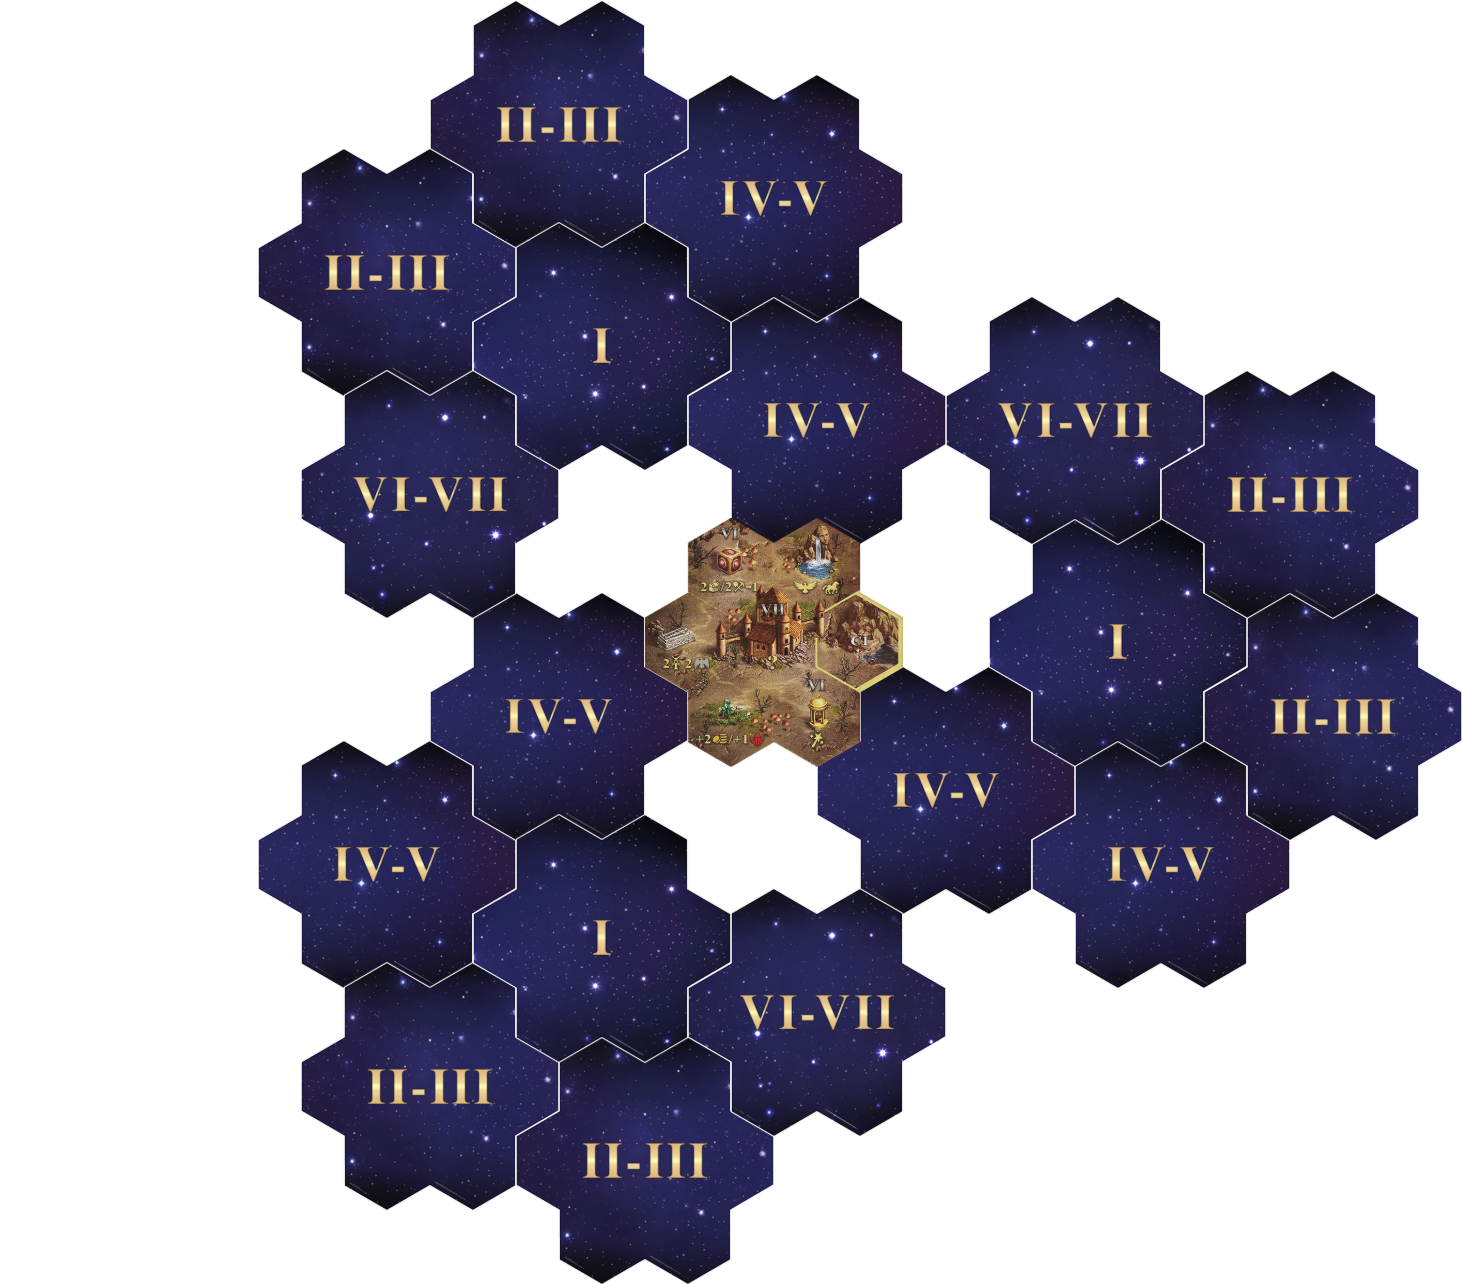
\includegraphics[width=0.85\linewidth]{\maps/dragon-valley-3p.png}
  \captionof{figure}{\textbf{3-PLAYER SCENARIO}}
  \vspace*{\fill}
  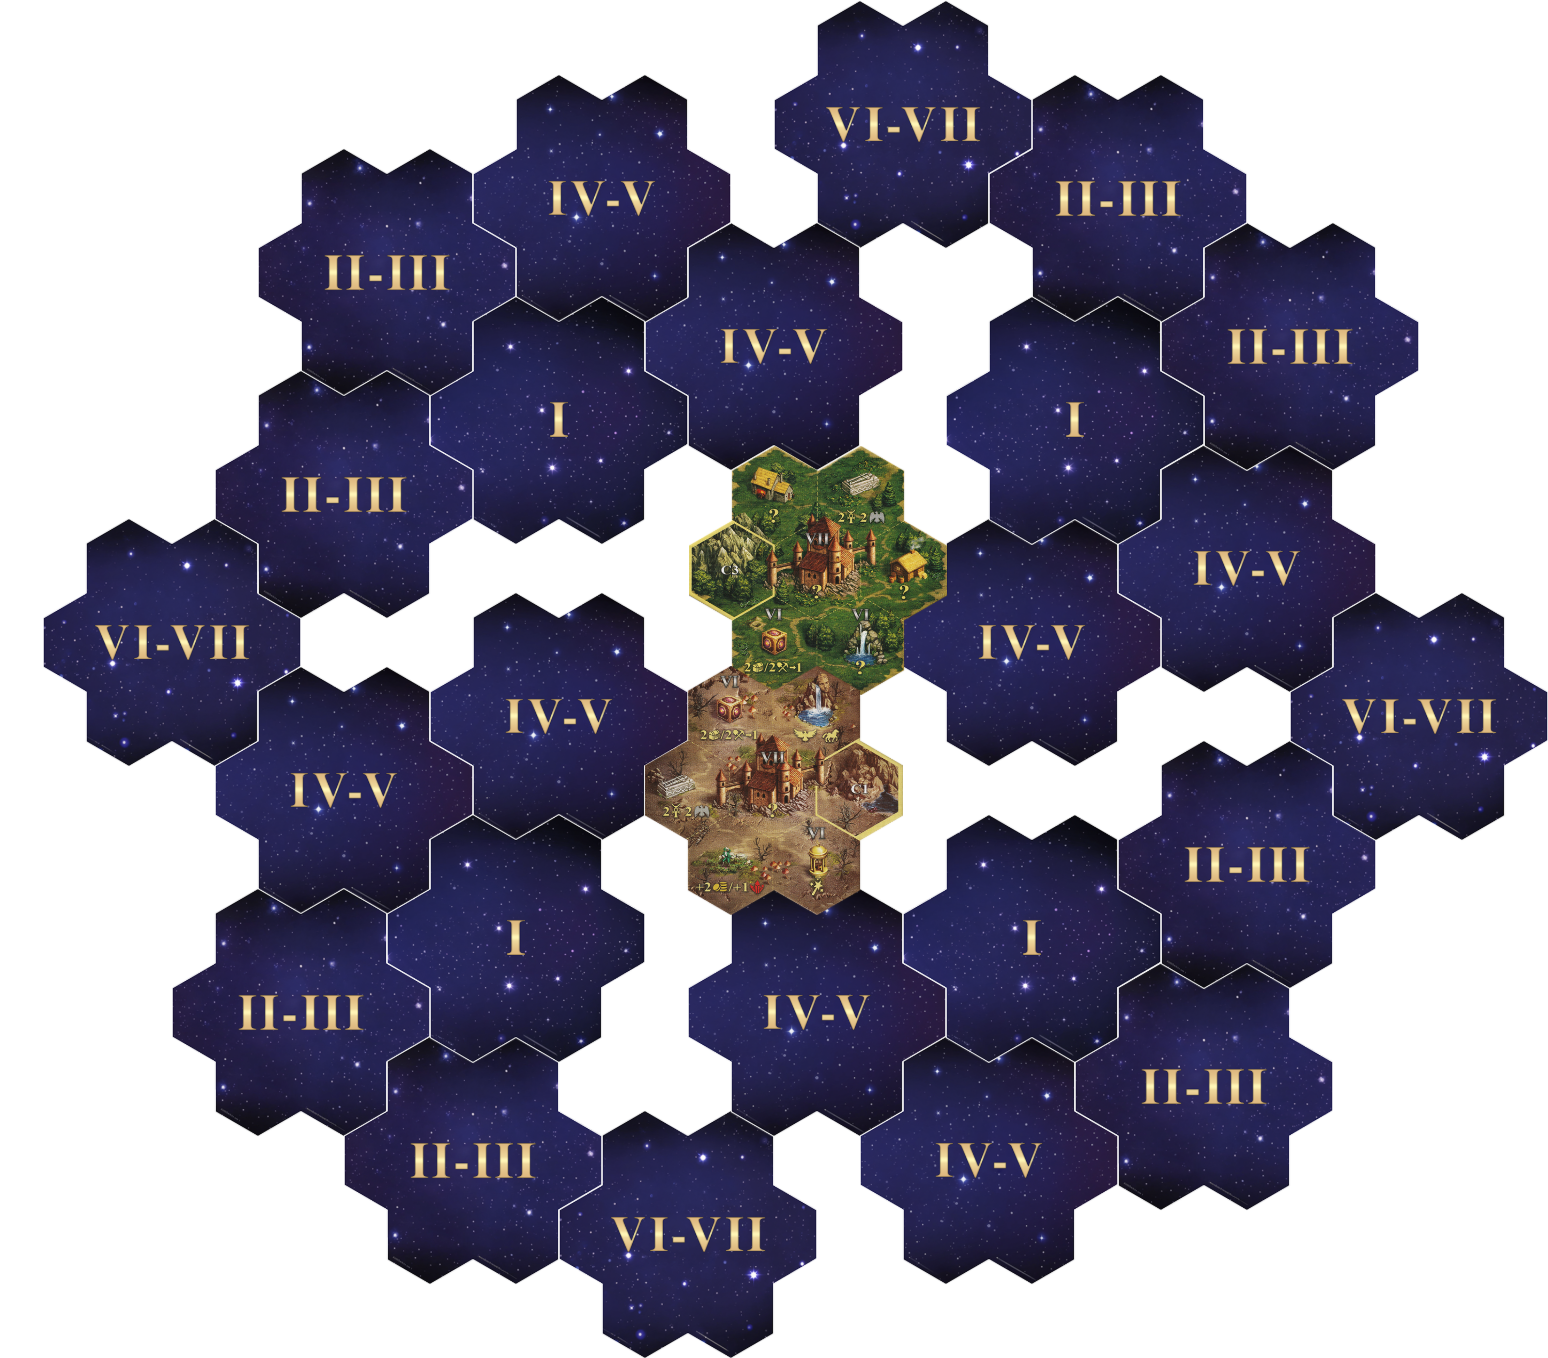
\includegraphics[width=1.15\linewidth]{\maps/dragon-valley-4p.png}
  \captionof{figure}{\textbf{4-PLAYER SCENARIO}}
\end{center}

\end{multicols*}
